\chapter{Practical Aspects}
\label{cha:practicalAspects}

To achieve my goal of creating Visual Bicycle Counter, I had to complete a few steps. With tools chosen, my work was to create a proper dataset for training ML model, train and evaluate this training to reach acceptable values of metrics I mentioned in section \ref{sec:theory}. After that, I could customize the API detection script to make it count cyclist rather than just detecting them using the trained model. Lastly, I used my edited script to run inference (detection) on other videos from a street camera on Lema Street and near ICE Krakow Congress Centre. I have prepared exemplary interpretation of how data obtained by my Visual Bicycle Counter can be used.
\section{Data Collection}
\label{sec:collection}
First of all I had to collect data. To accomplish that, on June 2020 I have created Virtual Machine (VM) with Ubuntu 18.04.5 Operating System (OS). Using Unix type OS was much easier and intuitive than using it on my Windows machine. After my VM was ready, steps to obtain video files from street camera stream were as follow:
\begin{enumerate}
    \item Installing ffmpeg for Ubuntu OS (from terminal):
    \begin{itemize}
        \item \colorbox{Gray}{sudo apt-get install ffmpeg}
    \end{itemize}
    \item Downloading and installing youtube-dl (from terminal):
    \begin{itemize}
        \item \colorbox{Gray}{sudo curl -L https://yt-dl.org/downloads/latest/youtube-dl -o /usr/local/bin/youtube-dl}
        \item \colorbox{Gray}{sudo chmod a+rx /usr/local/bin/youtube-dl}
    \end{itemize}
    \item Creating bash script that runs youtube-dl with proper parameters what is shown in Figure \ref{fig:script}
    \begin{figure}[H]
        \centering
        \resizebox{\textwidth}{!}{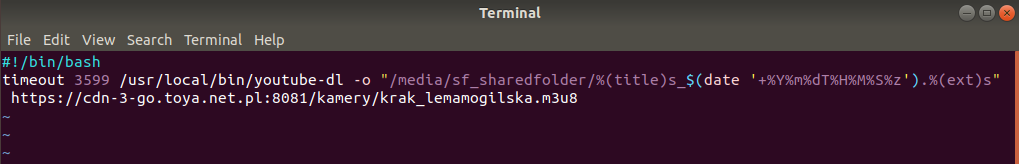
\includegraphics{images/bashScript}}
        \caption{This script runs youtube-dl, video files are saved to  directory with name containing stream name on http website and date of download. After 3599 seconds youtube-dl gets terminated.}
        \label{fig:script}
    \end{figure}
    \item Adding created script to \colorbox{Gray}{crontab -e} to schedule its execution to every hour as we can see in Figure below.
    \begin{figure}[H]
        \centering
        \resizebox{\textwidth}{!}{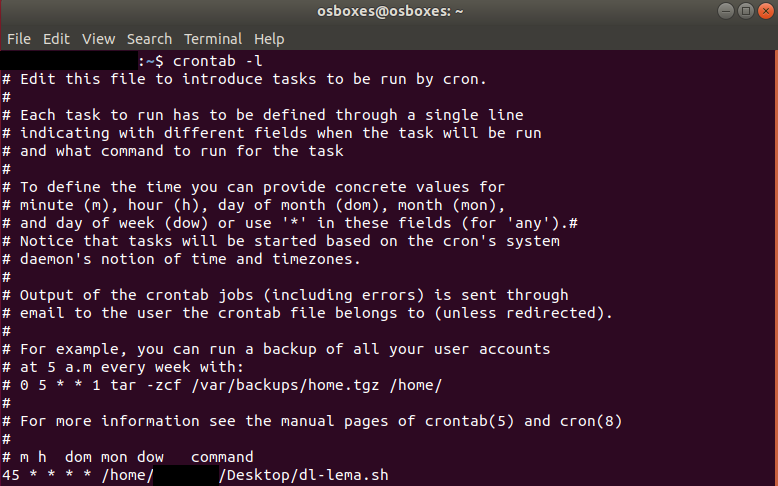
\includegraphics{images/crontabList}}
        \caption{output of \colorbox{Gray}{crontab -l} command which shows what commands execution was scheduled}
        \label{fig:crontabList}
    \end{figure}
\end{enumerate}
At this moment, downloading of video files proceeded automatically. Note that stable internet connection was very important as without it downloaded video files came out corrupted (damaged), what made them impossible to use later on.

\section{Creating the Dataset}
\label{sec: dataset}
After collecting enough videos I have started to create the dataset for training my YOLO model. This involved extracting frames from videos, choosing those with the most clear, visible cyclists, then manually labelling each image using LabelImg program and lastly divide labelled images on train and test data in ratio of approximately 8:2. To make it precise, those are steps I have taken:
\begin{enumerate}
    \item Frame extraction with VLC media player
    \begin{itemize}
        \item Scene Filter settings customization
        \newline \colorbox{Gray}{Tools -> Preferences -> Show settings -> All -> Video/Filters/Scene Filter}
        \begin{figure}[H]
            \centering
            \resizebox{\textwidth}{!}{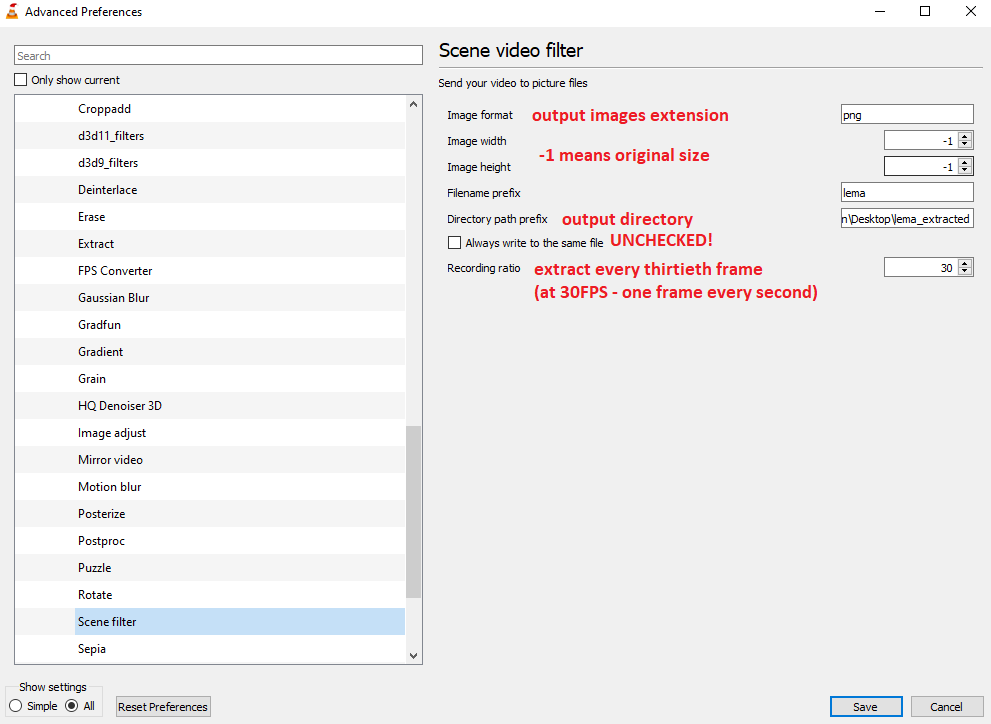
\includegraphics{images/vlc1}}
            \caption{Scene Filter edit window}
            \label{fig:vlc1}
        \end{figure}
        \item Switching Scene filter on
        \newline \colorbox{Gray}{Tools -> Preferences -> Show settings -> All -> Video/Filters -> check Scene video filter}
        \item Restart VLC and run video file with it (at this point frames are extracted automatically) 
    \end{itemize}
    \item Selection of frames (I used about 200 different frames with various count of cyclists on them)
    \item Manual frames labelling using LabelImg:
    \begin{itemize}
        \item after downloading LabelImg from repository, running it by executing command \colorbox{Gray}{python labelImg.py <images-path>} (Python3 or higher required) window shown in Figure \ref{fig:labelimg1} appears. It shows labelled image as well. To create label we simply click 
\includegraphics[scale=0.75]{images/button}
        \begin{figure}[H]
            \centering
            \resizebox{\textwidth}{!}{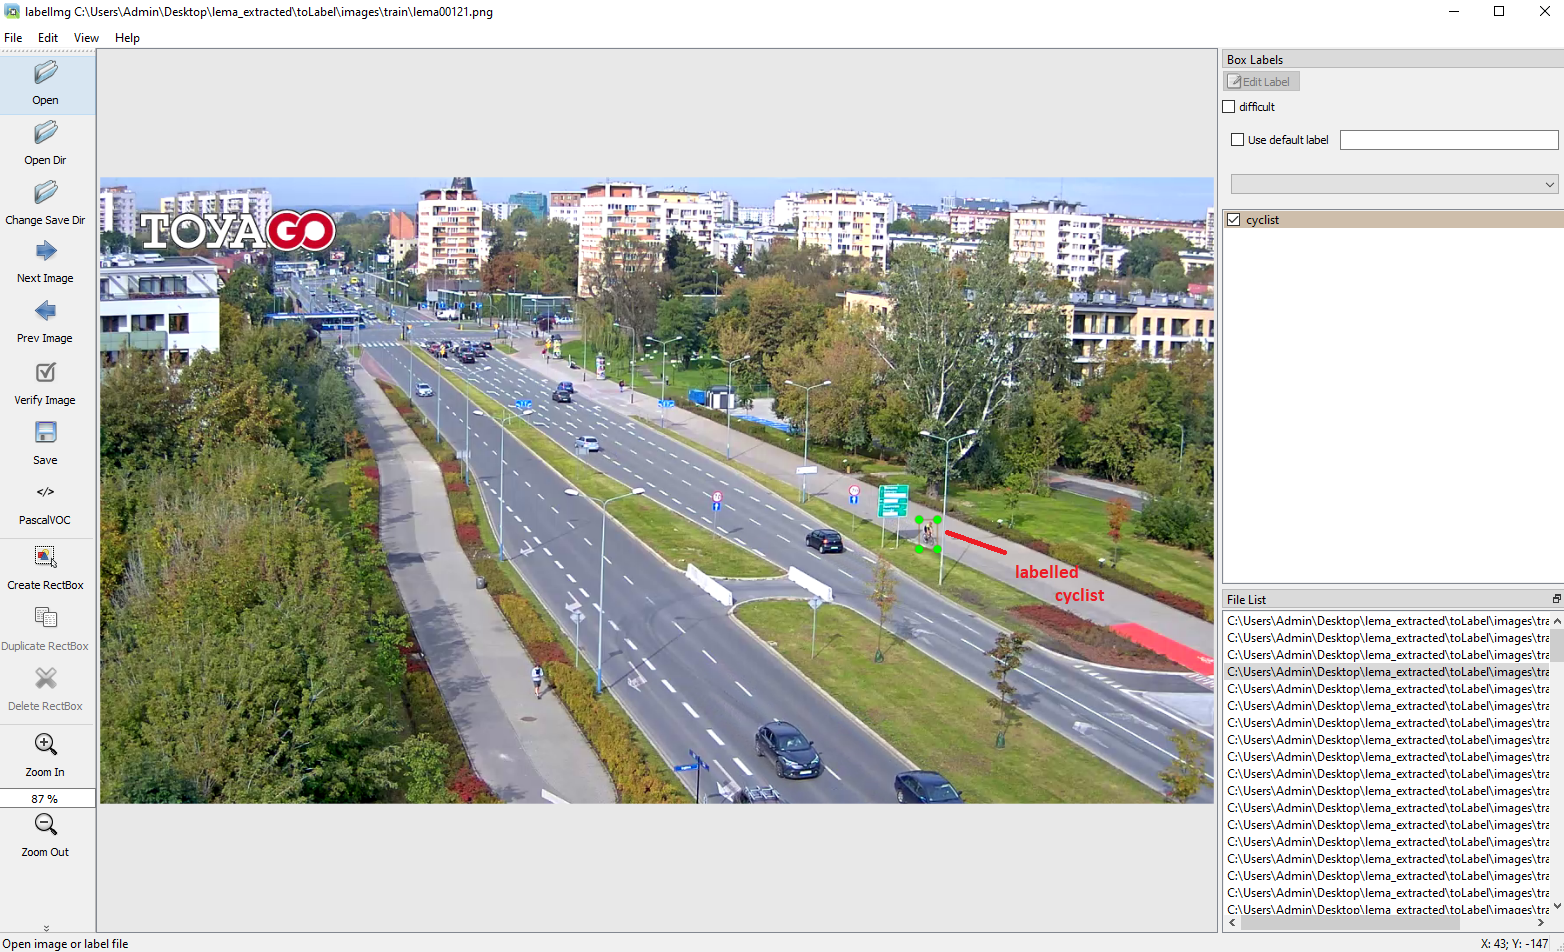
\includegraphics{images/labelImg}}
            \caption{LabelImg user interface with labelled image}
            \label{fig:labelimg1}
        \end{figure}
        Saving labelled frame will generate text file for this image with numeric label representation (one line in file for each label on image).
        \begin{figure}[H]
            \centering
            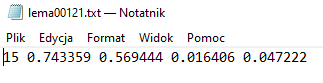
\includegraphics{images/text}
            \caption{Text file generated for image in Figure \ref{fig:labelimg1}}
            \label{fig:labelimg2}
        \end{figure}
    \end{itemize}
    \item Partition of images and corresponding text files on train and test (val) data. To accomplish and to do this easier I have written Python script which randomly divides images with text files to two directories "train" and "val" in desired ratio (in my case it was 80\% to train the model and 20\% to test it)
\end{enumerate}

\section{Environment Preparation, Training Model and Running Detection}
\label{sec:env}
As my working environment, I have chosen Google Colaboratory (GC) machine. It provides me with three times more GPU memory and overall better (faster) GPU device than the one in my computer, resulting in approximately six times faster training and detection processes. It was essential while performing inference (detection) because GC's machine made this operation execute close to real-time on 30 Frames Per Second (FPS) video files. My computer processed five frames per second while GC's machine processed almost 30 frames per second, what saved much time. Also, it turned out much more effective while running inference straight on the video stream from the website. Lastly, GC's machine has good Python3 support what facilitated the work. I have created Jupyter Notebook file to run code cells one by one, to speed up my work, what came especially handy while starting work on next day because sadly GC allows only a few hours of inactivity before restarting session and unsaved files are gone. To start training, I stored all necessary files like videos and labelled images on my Google Drive, connected to GC's machine. Also uploading files on the Drive and copying them on the machine was the fastest way to access my computer files. Training the model proceeded in few steps (Figures below will show code cells that have been run):
\begin{enumerate}
    \item After setting \colorbox{Gray}{runtime type} to GPU I mounted (connected) my Google Drive to GC's machine what creates a new directory on the machine named \colorbox{Gray}{gdrive} from which we can access Google Drive
    \newline \begin{figure} [h]
        \centering
        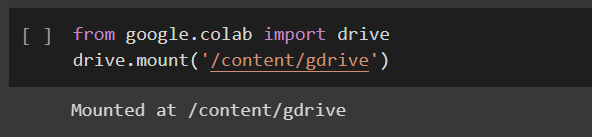
\includegraphics{images/train1}
        \caption{Mounting Drive}
        \label{fig:train1}
    \end{figure}
    \item Then I cloned YoloV5 GitHub repository
    \newline \begin{figure} [h]
        \centering
        \resizebox{\textwidth}{!}{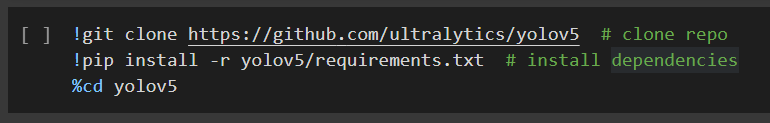
\includegraphics{images/train2}}
        \caption{Cloning repository to machine}
        \label{fig:train2}
    \end{figure}
    \item After that, I could run the training process with installed wandb for evaluating the model during and after training.
    \newline \begin{figure} [h]
        \centering
        \resizebox{\textwidth}{!}{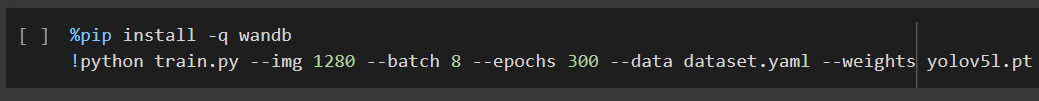
\includegraphics{images/train3}}
        \caption{Command used for training the model}
        \label{fig:train3}
    \end{figure}
    \newline Parameters used in command:
    \begin{itemize}
        \item img --- bigger of two numbers in video resolution
        \item batch --- how many images to process at once (limited by GPU memory --- in my case 8 was the biggest GPU could handle)
        \item epochs --- how many times to train the model on whole dataset
        \item data --- path to .yaml file which contains information about dataset
        \item weights --- path to weights file --- empty for training from scratch, I used pretrained weights of yolov5l model, which offers the best accuracy within my desired execution time (<40ms).
    \end{itemize}
\end{enumerate}

\section{Training Evaluation}
\label{sec:eval}
The first command from Figure \ref{fig:train3} installs wandb software on the machine. It automatically collects data during the training process and shows it in a more accessible manner --- charts. Below we can see how parameters mentioned in section \ref{sec:theory} (Recall, Precision and Loss) has been changing during the training process. Also, weights with the best combination of those three parameters (marked on charts) will be used for performing inference.
\begin{figure} [h]
    \centering
     \resizebox{\textwidth}{!}{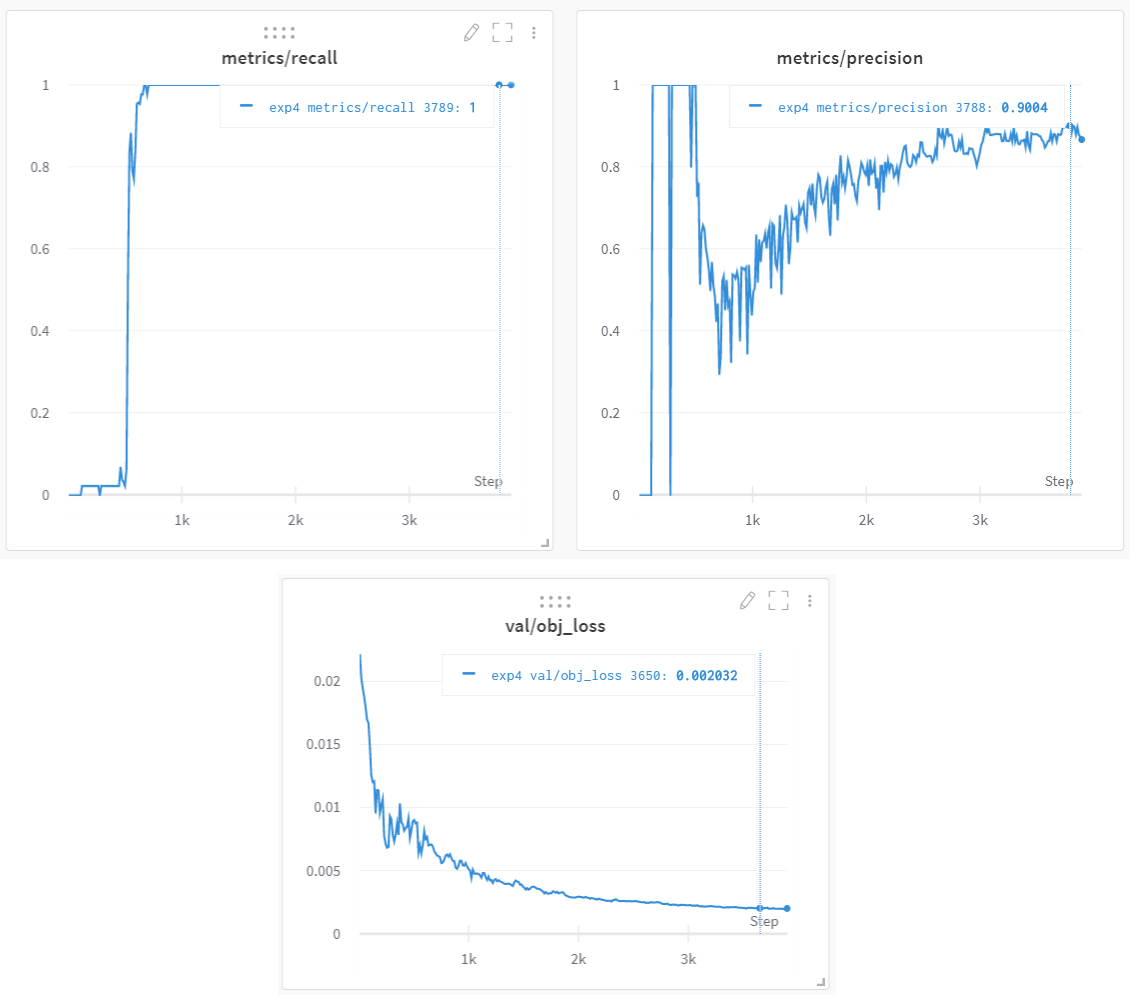
\includegraphics{images/eval1}}
    \caption{Changes of Recall, Precision and Loss during model training}
    \label{fig:eval1}
\end{figure}
\newline As we can see, parameters of trained model I have been using while performing inference on video files I have collected look as follows:
\begin{center}
    \begin{tabular}{ccc}
    Recall    & Precision     & Loss     \\
    1 (100\%) & 0.9004 (90\%) & 0.002032
    \end{tabular}
\end{center}
What basically means that every cyclist on test images was found (Recall), and 90\% of all detections are indeed cyclists (Precision). Also our model finds areas where detection is the most probable with very fast (Loss).

\section{Counter Implementation and Running Inference}
\label{sec:inference}
Running detection process is also really easy with YOLOv5 API, because it contains ready to use script \colorbox{Gray}{detect.py} that can be executed right away on video file or stream. Implementing counter was more of a challenge, because it is not implemented in API. I have chosen straight forward solution --- when a detected cyclist crosses a virtual line (on Figures \ref{fig:inference} and \ref{fig:inference5} shown as a green line drawn on video frames), counter value goes up. This approach was possible because of my Recall and Precision being on very good level. I knew every cyclist is detected on every frame of video (100\% Recall) and 90\% of detected objects are actually cyclists (Precision). Every script I have customized is put on public Github Repository \cite{repo}. Running detection process on GC's machine proceeded as follows:
\begin{enumerate}
    \item Mounting Google Drive on GC's machine
    \newline \begin{figure} [h]
        \centering
        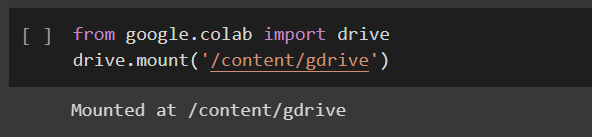
\includegraphics{images/train1}
        \caption{Mounting Drive}
        \label{fig:inference0}
    \end{figure}
    \item Copying model from Drive, unzipping it and installing required dependencies 
    \newline \begin{figure} [h]
        \centering
        \resizebox{\textwidth}{!}{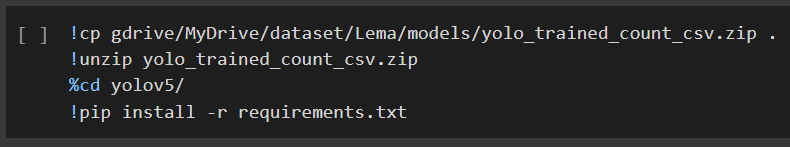
\includegraphics{images/inference1}}
        \caption{Installing ready API on machine}
        \label{fig:inference1}
    \end{figure}
    \item Uploading video for perform inference on it (two ways)
    \newline \begin{figure} [h]
        \centering
         \resizebox{\textwidth}{!}{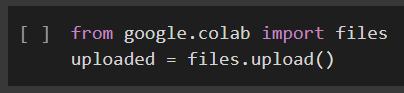
\includegraphics{images/inference2}}
        \caption{Uploading video file straight from local machine to GC's machine (slower)}
        \label{fig:inference2}
    \end{figure}
    \newline \begin{figure} [h]
        \centering
         \resizebox{\textwidth}{!}{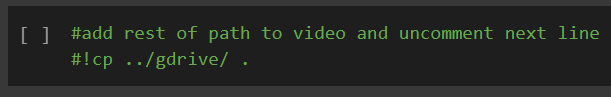
\includegraphics{images/inference3}}
        \caption{Copying video file from mounted drive after uploading video file to it (faster)}
        \label{fig:inference3}
    \end{figure}
    \item Running detection process
    \newline \begin{figure} [h]
        \centering
         \resizebox{\textwidth}{!}{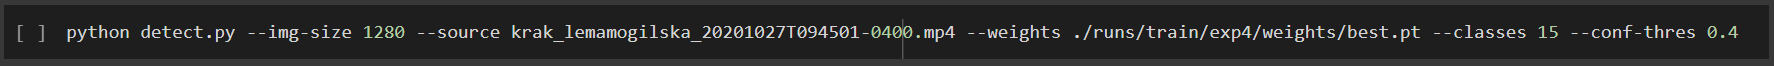
\includegraphics{images/inference4}}
        \caption{Command used for performing inference on video file using customized \colorbox{Gray}{detect.py} script}
        \label{fig:inference4}
    \end{figure}
    \newline Parameters used in command:
    \begin{itemize}
        \item img --- bigger of two numbers in video resolution
        \item source --- path to video file
        \item weights --- path to weights file (\colorbox{Gray}{best.pt} are best weights from training model) basically it is path to model we will use to detect cyclist
        \item classes --- identifier of detection classes to not filter out (\colorbox{Gray}{15} means that we only want to detect cyclists)
        \item conf --- confidence threshold value (probability that detected object is indeed cyclist) --- everything with higher confidence is considered as cyclist.
    \end{itemize}
\end{enumerate}
The Figures below shows a frame from a video after inference was performed with Counter already implemented (different cameras has counter line put on different place)
\begin{figure} [H]
    \centering
     \resizebox{\textwidth}{!}{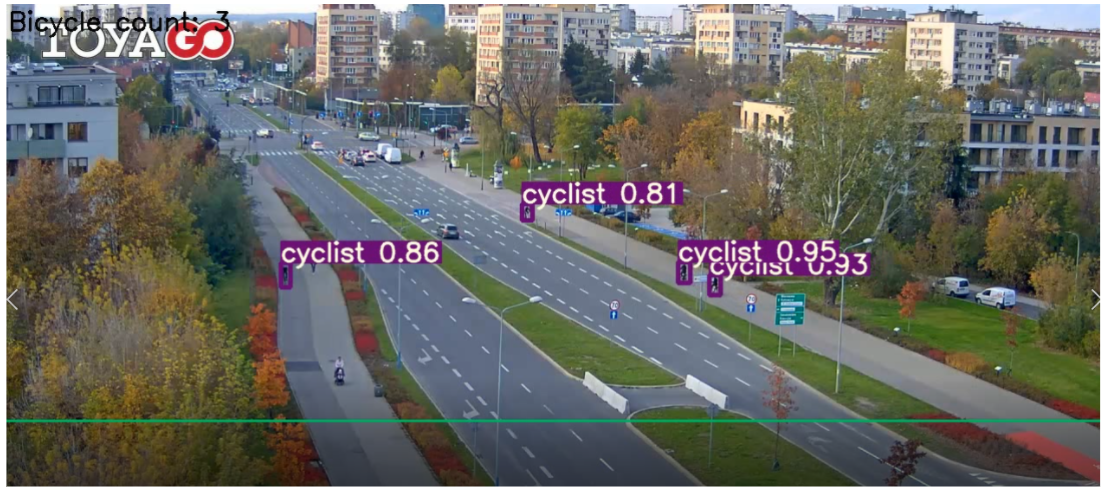
\includegraphics{images/inference}}
    \caption{Frame from video file generated during the detection process (inference performed on video file from camera on Lema Street)}
    \label{fig:inference}
\end{figure}
\begin{figure} [H]
    \centering
     \resizebox{\textwidth}{!}{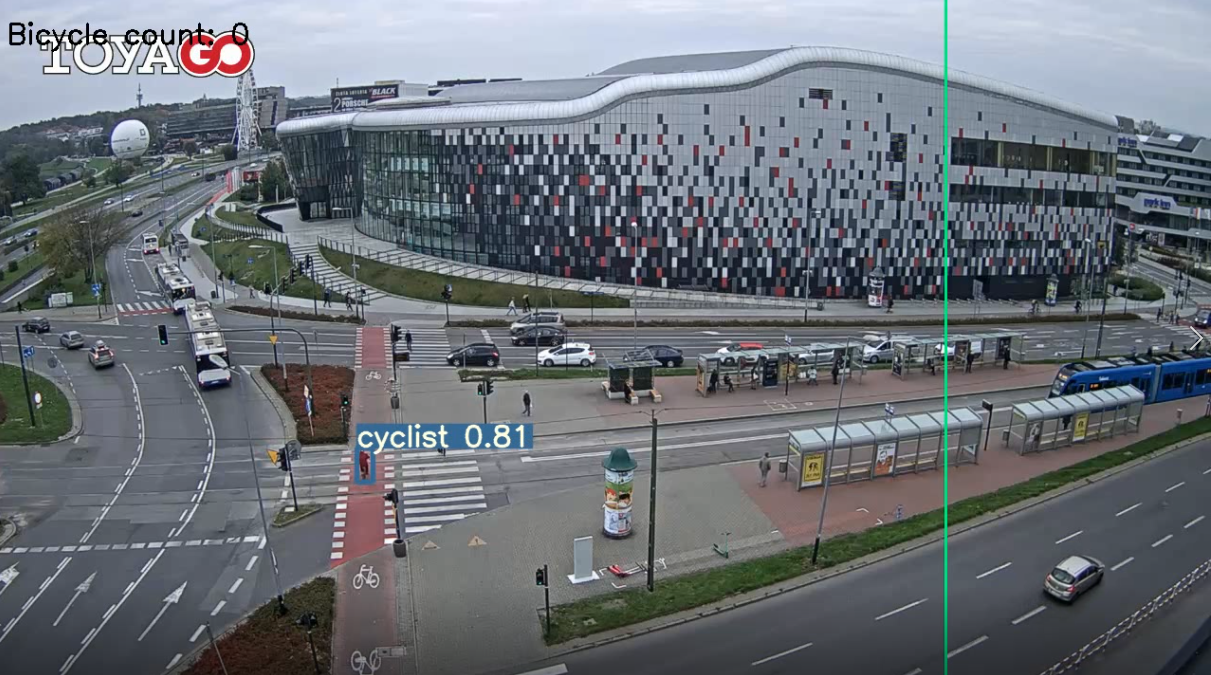
\includegraphics{images/inference5}}
    \caption{Frame from video file generated during the detection process (inference performed on video file from camera near ICE Krakow Congress Centre)}
    \label{fig:inference5}
\end{figure}
During the testing phase, I have been saving every video generated during the inference process. However, after that I quit doing that, because a generated video was almost five times bigger than the original one (1-hour video downloaded from website video stream was approximately 700MB big, so saving every result of inference would fill my Google Drive memory very quickly). Instead, I have implemented that at the end of execution of \colorbox{Gray}{detect.py} information about the video was written to \colorbox{Gray}{result.csv} file (video name, video duration, cyclist count).